\minpurp{Bindungen}
Namensbindung, Typbindung, Wertbindung, Adressbindung

anonym vs Namensbindung

statisch (zur Kompilezeit in Symboltabelle) vs dynamische Bindung (zur Laufzeit im Speicher z.B. Werte, virtuelle Methoden)

\minpurp{scope}
lexikalischer Scope: bindung an den umgebenden Block.

freie Variablen: keine lokale bindung (nicht in diesem Block)
Funktionen sind Closures wenn alle freien Variablen nicht-lokal gebunden sind

\minpurp{Speicherverwaltung}
Lebensdauer: \\
Global: unbegrenzt\\
Stack: allokation/freigabe mit funktionsaufruf/rückgabe\\
Heap: explizite reservierung/freigabe (Bei fehlern: Memory Leak/dangling reference)

\minmeth{Stack}
Aufbau Stackframe(x64 Windows): geregelt im ABI (Application Binary Interface):

Aufrufer erzeugt neuen Stackframe (groß genung für alle parameter) und lädt parameter. Aufbau:
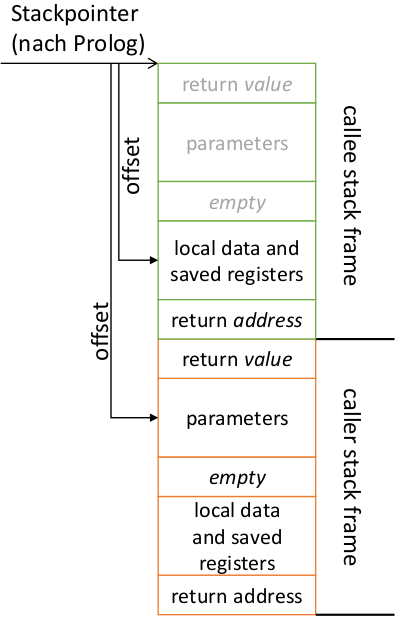
\includegraphics[angle=90,width=0.4\textwidth]{stack}

\minmeth{Heap}
Blöcke mit längenangaben, verkettet, werden nach ausreichend speicher durchsucht

\minmeth{Umgebung bei lokalen Funktionen}
\submeth{Statische Kette:} nichtlokale Variablen in darunterliegenden Stackframes, verfolgen von entsprechenden Pointern

\submeth{Closure:} wird bei übergabe/speichern von Funktion gebildet. Besteht aus Funktionszeiger und zeiger auf Heap-Objekt mit den gefangenen Variablen
Löst upward Funarg problem(Verweis auf nicht mehr existierende stackframes)
Bilden auch statische kette